\documentclass[12pt]{article}
\usepackage{mathtools,amssymb, amsthm, tikz}
\usetikzlibrary{intersections}
\usetikzlibrary{patterns}
\usetikzlibrary{arrows.meta}
\usepackage[margin=1in]{geometry}
\usepackage{url}
\usepackage{natbib}
\usepackage[colorlinks=true, linkcolor=black, urlcolor=blue, citecolor=blue]{hyperref}
\usepackage[T1]{fontenc}
\usepackage[magyar]{babel}
\usepackage[utf8]{inputenc}
\usepackage{lmodern}
\usepackage{fontspec}
\setmainfont{Times New Roman}
\usepackage{algorithm}
\usepackage{algpseudocode}

% Magyar pszeudokód

\renewcommand{\gets}{\textbf{:=}}

\makeatletter
\def\ALG@name{Algoritmus}
\makeatother
\algrenewcommand{\algorithmicdo}{\textbf{csináld}}
\algrenewcommand{\algorithmicfor}{\textbf{Ciklus}}
\algrenewcommand{\algorithmicrequire}{\textbf{Bemenet:}}
\algrenewcommand{\algorithmicensure}{\textbf{Kimenet:}}
\algrenewcommand{\algorithmicprocedure}{\textbf{Eljárás}}
\algrenewcommand{\algorithmicfunction}{\textbf{Függvény}}
\algrenewcommand{\algorithmicif}{\textbf{Ha}}
\algrenewcommand{\algorithmicthen}{\textbf{akkor}}
\algrenewcommand{\algorithmicelse}{\textbf{Különben}}
\algrenewcommand{\algorithmicwhile}{\textbf{amíg}}
\algtext{EndIf}{\textbf{Elágazás vége}}
\algtext{EndFor}{\textbf{Ciklus vége}}
\algtext{EndWhile}{\textbf{Ciklus vége}}
\algtext{EndProcedure}{\textbf{Eljárás vége}}

\title{Sutherland-Hodgman algoritmus}
\author{Pintér Bálint}
\renewcommand{\contentsname}{Tartalomjegyzék}
\renewcommand{\bibsection}{\section*{Források}}
\newcommand{\sokszog}{
    
\begin{tikzpicture}[scale=0.1, baseline=(current bounding box.center)]
        \draw[black] (3,4,4) -- (5, 3.6, 3.2) -- (5, 1.8, 2.6) -- (3,1,3) -- cycle;
    \end{tikzpicture}
}
\newcommand{\haromszog}{
    
\begin{tikzpicture}[scale=0.05, baseline=(current bounding box.center)]
        \draw[black] (8,3,2) -- (3,1,3) -- (3,4,4) -- cycle;
    \end{tikzpicture}
}
\newcommand{\kocka}{
    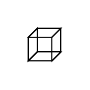
\begin{tikzpicture}[scale=0.15, baseline=(current bounding box.center)]
        \coordinate (O) at (0,0,0);
        \coordinate (A) at (0,2,0);
        \coordinate (B) at (0,2,2);
        \coordinate (C) at (0,0,2);
        \coordinate (D) at (2,0,0);
        \coordinate (E) at (2,2,0);
        \coordinate (F) at (2,2,2);
        \coordinate (G) at (2,0,2);

        \draw[black] (O) -- (C) -- (G) -- (D) -- cycle;
        \draw[black] (O) -- (A) -- (E) -- (D) -- cycle;
        \draw[black] (O) -- (A) -- (B) -- (C) -- cycle;
        \draw[black,opacity=0.8] (D) -- (E) -- (F) -- (G) -- cycle;
        \draw[black,opacity=0.6] (C) -- (B) -- (F) -- (G) -- cycle;
        \draw[black,opacity=0.8] (A) -- (B) -- (F) -- (E) -- cycle;
    \end{tikzpicture}
}


\begin{document}
\maketitle
\newpage
\tableofcontents
\newpage

\section{Bevezetés}
A Sutherland-Hodgman algoritmus egy clipping algoritmus. Feladata, hogy levágja
az alakzatok látómezőn kívül eső részeit. A teljesen kívül eső alakzatokat
elveti, a vágósíkokat metsző alakzatokat pedig úgy vágja meg, hogy csak a
látható rész maradjon. Fontos megjegyezni, hogy csak konvex vágótérrel
működik helyesen. A vágott sokszög lehet konkáv, de ilyenkor plusz feldolgozást igényelhet.
\begin{center}
    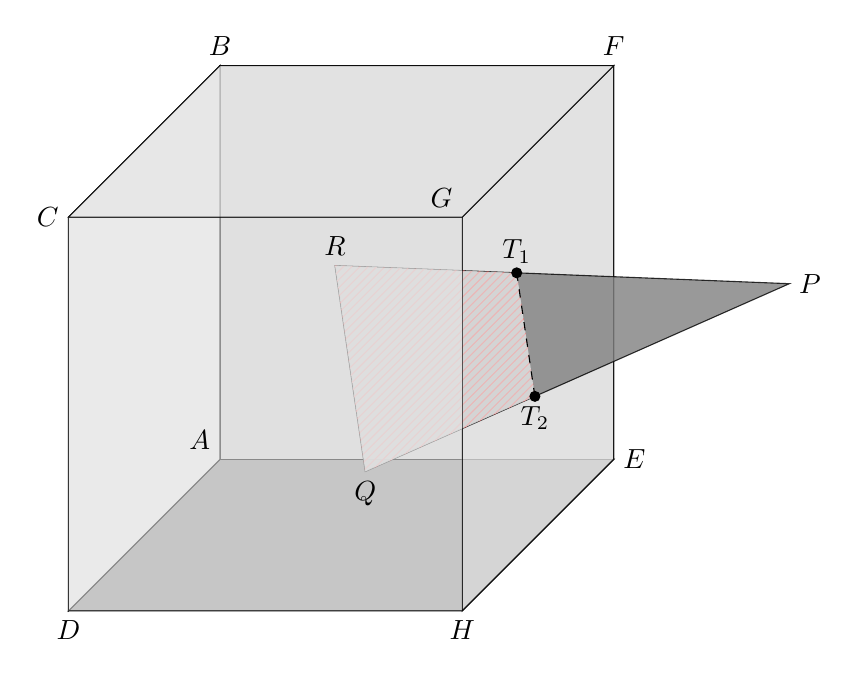
\begin{tikzpicture}
        \coordinate (A) at (0,0,0);
        \coordinate (B) at (0,5,0);
        \coordinate (C) at (0,5,5);
        \coordinate (D) at (0,0,5);
        \coordinate (E) at (5,0,0);
        \coordinate (F) at (5,5,0);
        \coordinate (G) at (5,5,5);
        \coordinate (H) at (5,0,5);

        \coordinate (P) at (8,3,2);
        \coordinate (Q) at (3,1,3);
        \coordinate (R) at (3,4,4);

        \coordinate (T1) at (5, 3.6, 3.2);
        \coordinate (T2) at (5, 1.8, 2.6);

        \draw[black,fill=gray!80] (A) -- (D) -- (H) -- (E) -- cycle; 		 % Alsó
        \draw[black,fill=gray!30] (A) -- (B) -- (F) -- (E) -- cycle; 		 % Hátsó
        \draw[black,fill=gray!10] (A) -- (B) -- (C) -- (D) -- cycle; 		 % Bal
        \draw[black,fill=gray!20,opacity=0.8] (E) -- (F) -- (G) -- (H) -- cycle; % Jobb
        \draw[black,fill=gray,opacity=0.8] (P) -- (Q) -- (R) -- cycle;
        \fill[pattern=north east lines, pattern color=red]
        (T1) -- (T2) -- (Q) -- (R) -- cycle;
        \fill[gray!20,opacity=0.8] (T1) -- (T2) -- (Q) -- (R) -- cycle;
        \draw[black,fill=gray!20,opacity=0.6] (D) -- (C) -- (G) -- (H) -- cycle; % Elülső
        \draw[black,fill=gray!20,opacity=0.8] (B) -- (C) -- (G) -- (F) -- cycle; % Felső
        \fill[black] (T1) circle (2pt);
        \fill[black] (T2) circle (2pt);
        \draw[black, dashed] (T1) -- (T2);

        \node[right] at (P) {$P$};
        \node[below] at (Q) {$Q$};
        \node[above] at (R) {$R$};
        \node[above] at (T1) {$T_{1}$};
        \node[below] at (T2) {$T_{2}$};
        \node[above left] at (A) {$A$};
        \node[above] at (B) {$B$};
        \node[left] at (C) {$C$};
        \node[below] at (D) {$D$};
        \node[right] at (E) {$E$};
        \node[above] at (F) {$F$};
        \node[above left] at (G) {$G$};
        \node[below] at (H) {$H$};

    \end{tikzpicture}
    \\
    \textbf{1. Ábra:}\\Sutherland-Hodgman algoritmus szemléltetése \\ $ABCDEFGH_{\kocka}$ vágótér\\$PQR_{\haromszog}$ Levágandó sokszög\\$RT_{1}T_{2}Q{\sokszog}$ Megvágott sokszög
\end{center}
\section{Az algoritmus}
\subsection{Vágótér (clip space)}
A levágást perspektív mátrixszal való szorzás után, de a $w$-vel való osztás
(perspective divide) előtt végezzük homogén koordinátákkal. Ez az úgynevezett
clip space. A perspektív mátrixszal való szorzás előtt a látótér egy csonkagúla
(viewing frustum). A perspektív mátrixszal való szorzás után a vágási
feltételek homogén koordinátákkal egy kocka határait adják meg. Így a vágás
feltételei egyszerűen vizsgálhatóak. Clip space-ben végezzük a levágást, mert
kameratérben a látótér egy csonkagúla, amire nehéz lenne vágni. A perspective
divide után a kamera mögötti pontok (melyekre $w<0$) helytelenül vetítődnek a
képernyőre, ezért a vágást a perspective divide előtt kell elvégezni.
\subsection{A vágás lépései}
Egy sokszöget a pontjai megadott sorrendje határozza meg. Az n csúcsú sokszög
oldalait a következőképpen képezzük a csúcsaiból:
\begin{align*}
    P_{n}P_{1},P_{1}P_{2},P_{2}P_{3},...,P_{n-1}P_{n}
\end{align*}
Az algoritmusunk vesz egy pontokból álló bemenetet (először a sokszög pontjai a bemenet), amelyet vág egy síkhoz, majd ennek a folyamatnak a kimenete lesz a következő síkhoz való vágásnak a bemenete. A sokszög oldalait
teszteljük a síkhoz képest. Az oldalnak négy lehetséges elhelyezkedése van a
síkhoz képest:
\begin{center}
    \begin{minipage}[t]{0.48\textwidth}
        \centering
        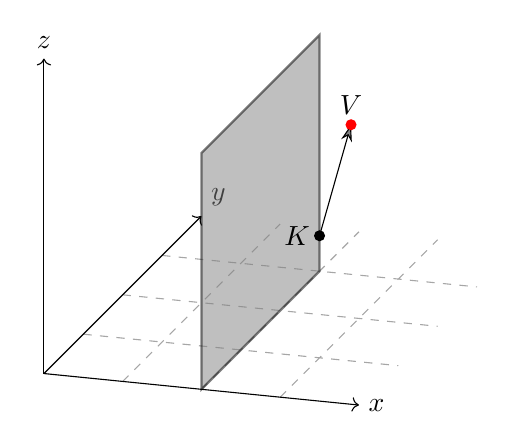
\begin{tikzpicture}[
                x={(1.00cm,-0.10cm)}, y={(0.50cm,0.50cm)}, z={(0cm,1.00cm)} ]

            \draw[gray, thin, dashed, opacity=0.7]
            \foreach \x in {1, 2, 3} {
                    (\x, 0, 0) -- (\x, 4, 0)
                }
            \foreach \y in {1, 2, 3} {
                    (0, \y, 0) -- (4, \y, 0)
                };

            \draw[->] (0,0,0) -- (4,0,0) node[right] {$x$};
            \draw[->] (0,0,0) -- (0,4,0) node[above right] {$y$};
            \draw[->] (0,0,0) -- (0,0,4) node[above] {$z$};

            \filldraw[
                draw=black,
                fill=gray,
                opacity=0.5,
                thick
            ]
            (2,0,0) -- (2,0,3) -- (2,3,3) -- (2,3,0) -- cycle;
            \coordinate (K) at (2.5,2,1);
            \coordinate (V) at (3.4,1,3);
            \draw[->, -{Stealth[length=6pt, width=4pt, fill=gray]}, name path=oldal] (K) -- (V);
            \fill[red] (V) circle (2pt);
            \fill[black] (K) circle (2pt);

            \node[left] at (K) {$K$};
            \node[above] at (V) {$V$};

        \end{tikzpicture}
        \vspace{0.5ex}
        \hspace*{4mm}
        \\\textbf{1. (BE$\rightarrow$BE) Mindkét pontja belül van.} \\ Csak a végpontot adjuk a kimenethez. (A kezdeti pontja már hozzá lett/lesz adva, amikor végpontként vizsgáljuk/vizsgáltuk.)
    \end{minipage}
    \hfill
    \begin{minipage}[t]{0.48\textwidth}
        \centering
        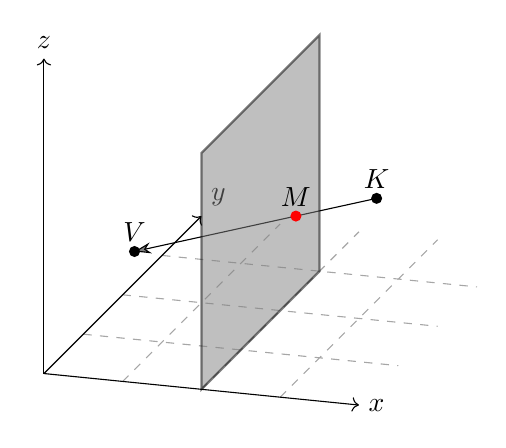
\begin{tikzpicture}[
                x={(1.00cm,-0.10cm)}, y={(0.50cm,0.50cm)}, z={(0cm,1.00cm)} ]

            \draw[gray, thin, dashed, opacity=0.7]
            \foreach \x in {1, 2, 3} {
                    (\x, 0, 0) -- (\x, 4, 0)
                }
            \foreach \y in {1, 2, 3} {
                    (0, \y, 0) -- (4, \y, 0)
                };

            \draw[->] (0,0,0) -- (4,0,0) node[right] {$x$};
            \draw[->] (0,0,0) -- (0,4,0) node[above right] {$y$};
            \draw[->] (0,0,0) -- (0,0,4) node[above] {$z$};

            \coordinate (K) at (2.5,3.45,0.75);
            \coordinate (V) at (1,0.3,1.5);
            \draw[->, -{Stealth[length=6pt, width=4pt, fill=gray]}] (K) -- (V);

            \filldraw[
                draw=black,
                fill=gray,
                opacity=0.5,
                thick
            ]
            (2,0,0) -- (2,0,3) -- (2,3,3) -- (2,3,0) -- cycle;
            \coordinate (M) at (2,2.4,1);
            \fill[black] (V) circle (2pt);
            \fill[black] (K) circle (2pt);
            \fill[red] (M) circle (2pt);

            \node[above] at (K) {$K$};
            \node[above] at (V) {$V$};
            \node[above] at (M) {$M$};

        \end{tikzpicture}
        \vspace{0.5ex}
        \hspace*{4mm}
        \\\textbf{2. (BE$\rightarrow$KI) Kezdeti pontja belül van, de a végpontja kívül van.}\\ Az oldal és a sík metszéspontját adjuk a kimenethez.
    \end{minipage}

    \vspace{1cm}
    \begin{minipage}[t]{0.48\textwidth}
        \centering
        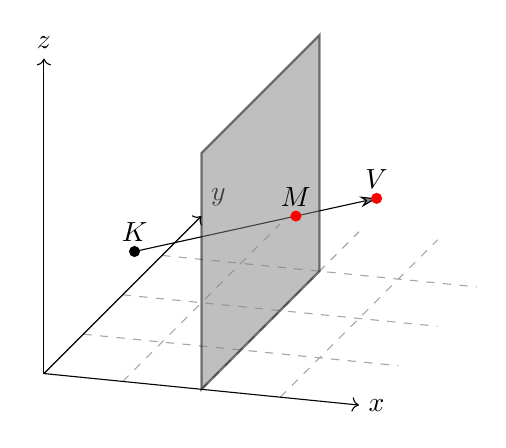
\begin{tikzpicture}[
                x={(1.00cm,-0.10cm)}, y={(0.50cm,0.50cm)}, z={(0cm,1.00cm)} ]

            \draw[gray, thin, dashed, opacity=0.7]
            \foreach \x in {1, 2, 3} {
                    (\x, 0, 0) -- (\x, 4, 0)
                }
            \foreach \y in {1, 2, 3} {
                    (0, \y, 0) -- (4, \y, 0)
                };

            \draw[->] (0,0,0) -- (4,0,0) node[right] {$x$};
            \draw[->] (0,0,0) -- (0,4,0) node[above right] {$y$};
            \draw[->] (0,0,0) -- (0,0,4) node[above] {$z$};

            \coordinate (V) at (2.5,3.45,0.75);
            \coordinate (K) at (1,0.3,1.5);
            \draw[->, -{Stealth[length=6pt, width=4pt, fill=gray]}] (K) -- (V);

            \filldraw[
                draw=black,
                fill=gray,
                opacity=0.5,
                thick
            ]
            (2,0,0) -- (2,0,3) -- (2,3,3) -- (2,3,0) -- cycle;
            \coordinate (M) at (2,2.4,1);
            \fill[red] (V) circle (2pt);
            \fill[black] (K) circle (2pt);
            \fill[red] (M) circle (2pt);

            \node[above] at (K) {$K$};
            \node[above] at (V) {$V$};
            \node[above] at (M) {$M$};
        \end{tikzpicture}
        \vspace{0.5ex}
        \hspace*{4mm}
        \\\textbf{3. (KI$\rightarrow$BE) Kezdeti pontja kívül van, de a végpontja belül van.}\\ A körüljárási irány megtartása érdekében először az oldal és a sík metszéspontját, majd a végpontot adjuk hozzá a kimenethez.
    \end{minipage}
    \hfill
    \begin{minipage}[t]{0.48\textwidth}
        \centering
        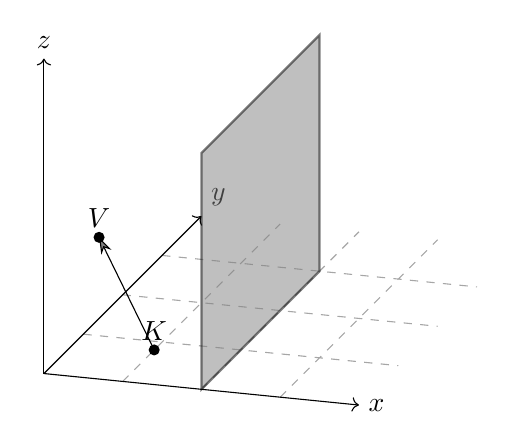
\begin{tikzpicture}[
                x={(1.00cm,-0.10cm)}, y={(0.50cm,0.50cm)}, z={(0cm,1.00cm)} ]

            \draw[gray, thin, dashed, opacity=0.7]
            \foreach \x in {1, 2, 3} {
                    (\x, 0, 0) -- (\x, 4, 0)
                }
            \foreach \y in {1, 2, 3} {
                    (0, \y, 0) -- (4, \y, 0)
                };

            \draw[->] (0,0,0) -- (4,0,0) node[right] {$x$};
            \draw[->] (0,0,0) -- (0,4,0) node[above right] {$y$};
            \draw[->] (0,0,0) -- (0,0,4) node[above] {$z$};

            \coordinate (V) at (0.2,1,1.25);
            \coordinate (K) at (1,0.8,0);
            \draw[->, -{Stealth[length=6pt, width=4pt, fill=gray]}] (K) -- (V);

            \filldraw[
                draw=black,
                fill=gray,
                opacity=0.5,
                thick
            ]
            (2,0,0) -- (2,0,3) -- (2,3,3) -- (2,3,0) -- cycle;
            \fill[black] (V) circle (2pt);
            \fill[black] (K) circle (2pt);

            \node[above] at (K) {$K$};
            \node[above] at (V) {$V$};
        \end{tikzpicture}
        \vspace{0.5ex}
        \hspace*{4mm}
        \\\textbf{4. (KI$\rightarrow$KI) Mindkét pontja kívül van.} \\Nem adunk semmit a kimenethez.
    \end{minipage}
    \textbf{2.~Ábra}
    \\
    \begin{tabular}{l @{} l}
        \textbf{K} - & Kezdőpont   \\
        \textbf{V} - & Végpont     \\
        \textbf{M} - & Metszéspont \\
    \end{tabular}
    \\
    A pirossal jelölt pontok lesznek hozzáadva a kimenethez
\end{center}
A pontokról clip space-ben egyszerű elsőfokú egyenlőtlenséggel el lehet dönteni, hogy a sík
melyik oldalán van (mivel egy kocka). A perspektív mátrixunk úgy lett megírva,
hogy $x,y\in[-1;1]$ és $z\in[0;1]$. A perspective divide előtt ($w$-vel osztás) a koordinátáink:
\begin{align*}
    -w & \leq x \leq w \\
    -w & \leq y \leq w \\
    0  & \leq z \leq w \\
\end{align*}
Így a feltételeink a kocka különböző oldalaira:
\begin{center}
    \begin{tabular}{|c | c | c |}
        \hline
        % Top alignment [t] added to all \parbox commands
        \parbox[t]{0.25\linewidth}{
            \textbf{Jobb oldali sík:}
            \[
                \begin{aligned}
                    x & \leq w     \\
                    0 & \leq w - x
                \end{aligned}
            \]
        } &
        \parbox[t]{0.25\linewidth}{
            \textbf{Felső oldal síkja:}
            \[
                \begin{aligned}
                    y & \leq w     \\
                    0 & \leq w - y
                \end{aligned}
            \]
        } &
        \parbox[t]{0.25\linewidth}{
            \textbf{Távoli oldal síkja:}
            \[
                \begin{aligned}
                    z & \leq w     \\
                    0 & \leq w - z
                \end{aligned}
            \]
        }   \\
        \hline
        \parbox[t]{0.25\linewidth}{
            \textbf{Bal oldali sík:}
            \[
                \begin{aligned}
                    -w & \leq x     \\
                    0  & \leq x + w
                \end{aligned}
            \]
        } &
        \parbox[t]{0.25\linewidth}{
            \textbf{Alsó oldal síkja:}
            \[
                \begin{aligned}
                    -w & \leq y     \\
                    0  & \leq y + w
                \end{aligned}
            \]
        } &
        \parbox[t]{0.25\linewidth}{
            \textbf{Közeli oldal síkja:}
            \[
                \begin{aligned}
                    0 & \leq z
                \end{aligned}
            \]
        }   \\
        \hline
    \end{tabular}
\end{center}
Ezek a feltételek egyben megadják a síktól való távolságot is, amikkel ki tudjuk számolni a metszéspontokat a két pont interpolálásával.
\newpage
\section{Pszeudokód}
Az alap Sutherland-Hodgman algoritmus:
\begin{algorithm}
    \caption{Sutherland-Hodgman algoritmus}
    \begin{algorithmic}[1]

        \State $\text{kimenetiLista} \gets \text{eredetiSokszog}$

        \For{\textbf{minden} $\text{vagasiEl} \in \text{vagoSokszog}$}
        \State $\text{bemenetiLista} \gets \text{kimenetiLista}$
        \State $\text{kimenetiLista} \gets \emptyset$

        \For{$i \gets 1$ \textbf{tól} $\text{bemenetiListaHossz}$ \textbf{ig}}
        \State $\text{aktualisPont} \gets \text{bemenetiLista}[i]$
        \State $\text{elozoPont} \gets \text{bemenetiLista}[(i-2) \bmod \text{bemenetiListaHossz}+1]$
        \State $\text{metszesPont} \gets \text{SzamolMetszespont}(\text{elozoPont}, \text{aktualisPont}, \text{vagasiEl})$

        \If{$\text{aktualisPont}$ belül van $\text{vagasiEl}$}
        \If{$\text{elozoPont}$ nincs belül $\text{vagasiEl}$}
        \State $\text{kimenetiLista.hozzaad}(\text{metszesPont})$
        \EndIf
        \State $\text{kimenetiLista.hozzaad}(\text{aktualisPont})$
        \ElsIf{$\text{elozoPont}$ belül van $\text{vagasiEl}$}
        \State $\text{kimenetiLista.hozzaad}(\text{metszesPont})$
        \EndIf
        \EndFor
        \EndFor
    \end{algorithmic}
\end{algorithm}
\newpage
\nocite{*}
\bibliographystyle{plainnat}
\bibliography{forrasok}

\end{document}